\section{Introduction}
In genomic analyses, it is commonly of interest to assess whether
there is enrichment of one set of features near another in the
linear genome, or to assess correlation across samples for pairs of
genomic features assayed for different modalities (e.g. RNA,
accessibility) \citep{reviewdilemma2014}.
For example, enrichment of accessibility peaks near sets of genes may
indicate a regulatory relationship \citep{lee2020fluent}, while
enrichment of genetic variants associated with phenotype near
tissue-specific accessibility may point to mechanisms of the inherited
risk.
Such analyses often rely on a null distribution, and one strategy for
generating a null distribution is to permute or shuffle the
genomic features -- giving random positions drawn uniformly along the
genome to existing features, possibly while considering an exclusion
list of regions where features should not be located.
Uniformly distributed ``null feature sets'' will not generally exhibit
natural clumping properties of
genomic feature sets where there often exists a complex
dependency structure, both in terms of placement and correlation of
metadata (signal strength, cell-type-specificity, etc.).
Using an overly simplistic null feature set that doesn't take into
account local dependency of features and metadata could result in
misleading conclusions.
Some more sophisticated methods exist, for example
GAT, which additionally allows for controlling feature placement with
respect to local GC content
\citep{GAT_2013}, and regioneR, which implements a circular chromosome
shift to preserve inter-feature distance \citep{gel2016regioner}.

The block bootstrap \citep{politis1999subsampling}
provides an alternative to random starts, where one instead generates
random feature sets by sampling large blocks of features within the
segments from the original set with replacement, as proposed for genomic data
by \citet{bickel2010subsampling}.
Generating new genomic feature sets via the block bootstrap is more
computationally intensive than a per-feature random start assignment.
To address this, GSC \citep{bickel2010subsampling} implements a
strategy of swapping pairs of blocks in order to generate a bootstrap
distribution while avoiding generation of a genome-scale bootstrap
sample.

Here we describe the \bootranges software, which uses efficient
vectorized code for performing block bootstrap sampling of
\granges \citep{lawrence2013software} objects with the Bioconductor
ecosystem.
\bootranges is part of a modular analysis workflow, where bootstrapped
\granges generated by \bootranges can then be analyzed at block or
genome level using tidy downstream pipelines with \plyranges
\citep{lee2019plyranges}.
Here we demonstrate \bootranges, and additionally provide
recommendations for genome segmentation and block length.
We demonstrate how \bootranges can be incorporated into complex
downstream analyses, for example to avoid arbitrary thresholds when
comparing differentially expressed genes and differentially accessible
peaks.

\vspace*{-20pt}

\section{Features}
The schematic diagram of a block bootstrap, and the workflow of \bootranges in combination with \plyranges is provided in \cref{fig:framework}. \bootranges offers a simple ``unsegmented'' as well as a ``segmented'' block bootstrap:
%A common assumption made of evolutionary path that there are global shits in base composition indicates segmenting DNA sequence into a number of large statistically homogeneous regions within which to block bootstrap features gives a better fit to the data.
since the distribution of features in the genome is not uniform, we follow the logic of \citet{bickel2010subsampling} and consider to perform block bootstrapping within segments of the genome, which are more homogeneous in terms of base composition and inter-feature distance.
We consider various genome segmentation procedures(e.g. based on gene density ) or annotations(e.g. Giemsa bands, 
Segway segments \citep{hoffman:Segway}, or ChromHMM segments\citep{ernst2012chromhmm}), defining a number of large (e.g. on the order of megabase pairs), relatively homogeneous segments within which to block bootstrap features.
% Segments can be derived, e.g. based on gene density 
% or given as known segments, e.g. Giemsa bands, 
% Segway segments \citep{hoffman:Segway}, or ChromHMM segments\citep{ernst2012chromhmm}. 
The \granges objects are taken as the inputs for feature \bm{$x$} and \bm{$y$} with optional metadata columns used for computing a test statistic. Given segmentation method and block length, a \bootranges object of \bm{$y$} is generated, which is a \granges object with all the ranges concatenated, and iteration, blocks and block length indicated by metadata columns. 
After deriving the bootstrap distribution of test statistics, an empirical p-value, the number of times that show an equal or greater statistics than the observed statistic, or any types of intervals can be reported for testing the null hypothesis that there is no true biological relevant association between features. 
The \bootranges implementing algorithms are explained schematically in Supplementary \cref{sec:algorithm}.

\vspace{-0.3cm}
\begin{figure}[htbp]
\centering% default with `floatrow`
\setlength{\abovecaptionskip}{-0.05cm}
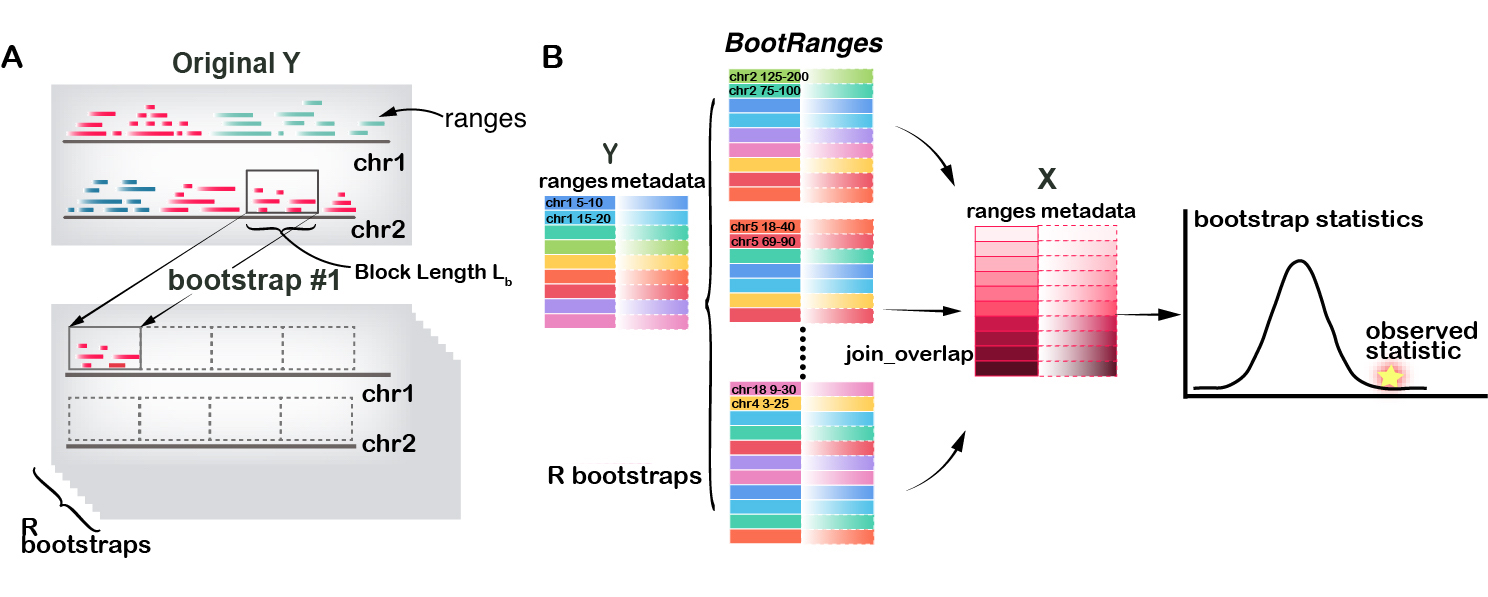
\includegraphics[scale=0.65]{Figures/bootRanges.jpg}
\caption{Overview of \textit{airpart} framework. (a) The schematic diagram of \bootranges with blockLength $L_b$ across chromosome. 
(b) 
%The workflow of \bootranges. 
Feature \bm{$x$} is overlapped with feature \bm{$y$} and bootRanges using \emph{plyranges} join\_overlap function
to derive 
the the observed statistic and bootstrap distribution of interested statistics.}
\label{fig:framework}
\vspace{-0.5cm}
\end{figure}

\vspace*{-20pt}
\section{Application}
First, \bootranges was evaluated on if there was significant overlap between caQTLs in human liver tissue and SNPs associated with total cholesterol \citep{CURRIN20211169}.
\cref{fig:result}A shows various segmentation method and block length effect on overlap rate distribution. Here overlap rate was defined as the proportion of SNPs across genome overlapping with peaks within 10kb. The fact that the estimated statistics variance increase at large $L_b$ indicated data were inhomogeneous and segmentation
% using either hidden Markov model(HMM) or circular binary search(CBS) \citep{cbs}
could alleviate the scenario. The exceptional decreasing trend using ChromHMM annotations for Roadmap Epigenomics indicated too many short segments failed to random swap the block genome when $L_b$ close to $L_s$. 
Regarding the choice of genome segmentation and of block length selection, we considered a number of diagnostic statistics including those recommended by \citet{bickel2010subsampling}: the variance of the null distribution of test statistics (\cref{fig:result}A) and a scaled version of the change in the width of the test statistic as $L_b$ changes; as well as examination of the inter-feature distance distribution (see Supplementary Methods).
After evaluation, $L_b \in [300000,600000]$ was shown to be a good range for carfully defined null distribution(\cref{fig:suppfig}A-C). 
More details were given in Supplementary \cref{sec:results}.

% One is trying to find $L_b$ that has the minimum value of a pseudostatistic $d^*(v)=|\sqrt{\frac{L_{v-1}}{L_v}}IQR(\mathcal{L}_{L_v})-IQR(\mathcal{L}_{L_{v-1}})|$ followed \citet{bickel2010subsampling}, where $\mathcal{L}_{L_v}$ is the statistic distribution at length $L_v$, $v=1,2,\cdots,V$ and $IQR(\mathcal{L})$ is the interquartile range.
% \cref{fig:suppfig}A showed $d^*$ were in common had smaller values when $L_b\in[300000,800000]$. Another way was evaluating conversing spatial distribution by assuming generated null sets have similar properties with original sets, eg. inter-feature distance. The Earth Mover's Distance (EMD) was used to access two distribution similarity because it is proportional to the minimum amount of work required to change one distribution into the other. Since the EMD always decreased as $L_b$ increased as more neighbouring features were reserved, the right $L_b$ should be chosen that a longer length won’t improve much as well as requesting $L_b$ is much smaller than the $L_s$. So [200000,600000] was shown to be  a good range by visualization and according to the Elbow Method of EMD(\cref{fig:suppfig}B-C). 

%\vspace{-0.5cm}
\begin{figure}[hbtp]
\centering% default with `floatrow`
\setlength{\abovecaptionskip}{-0.1cm}
\setlength{\belowcaptionskip}{-0.1cm}
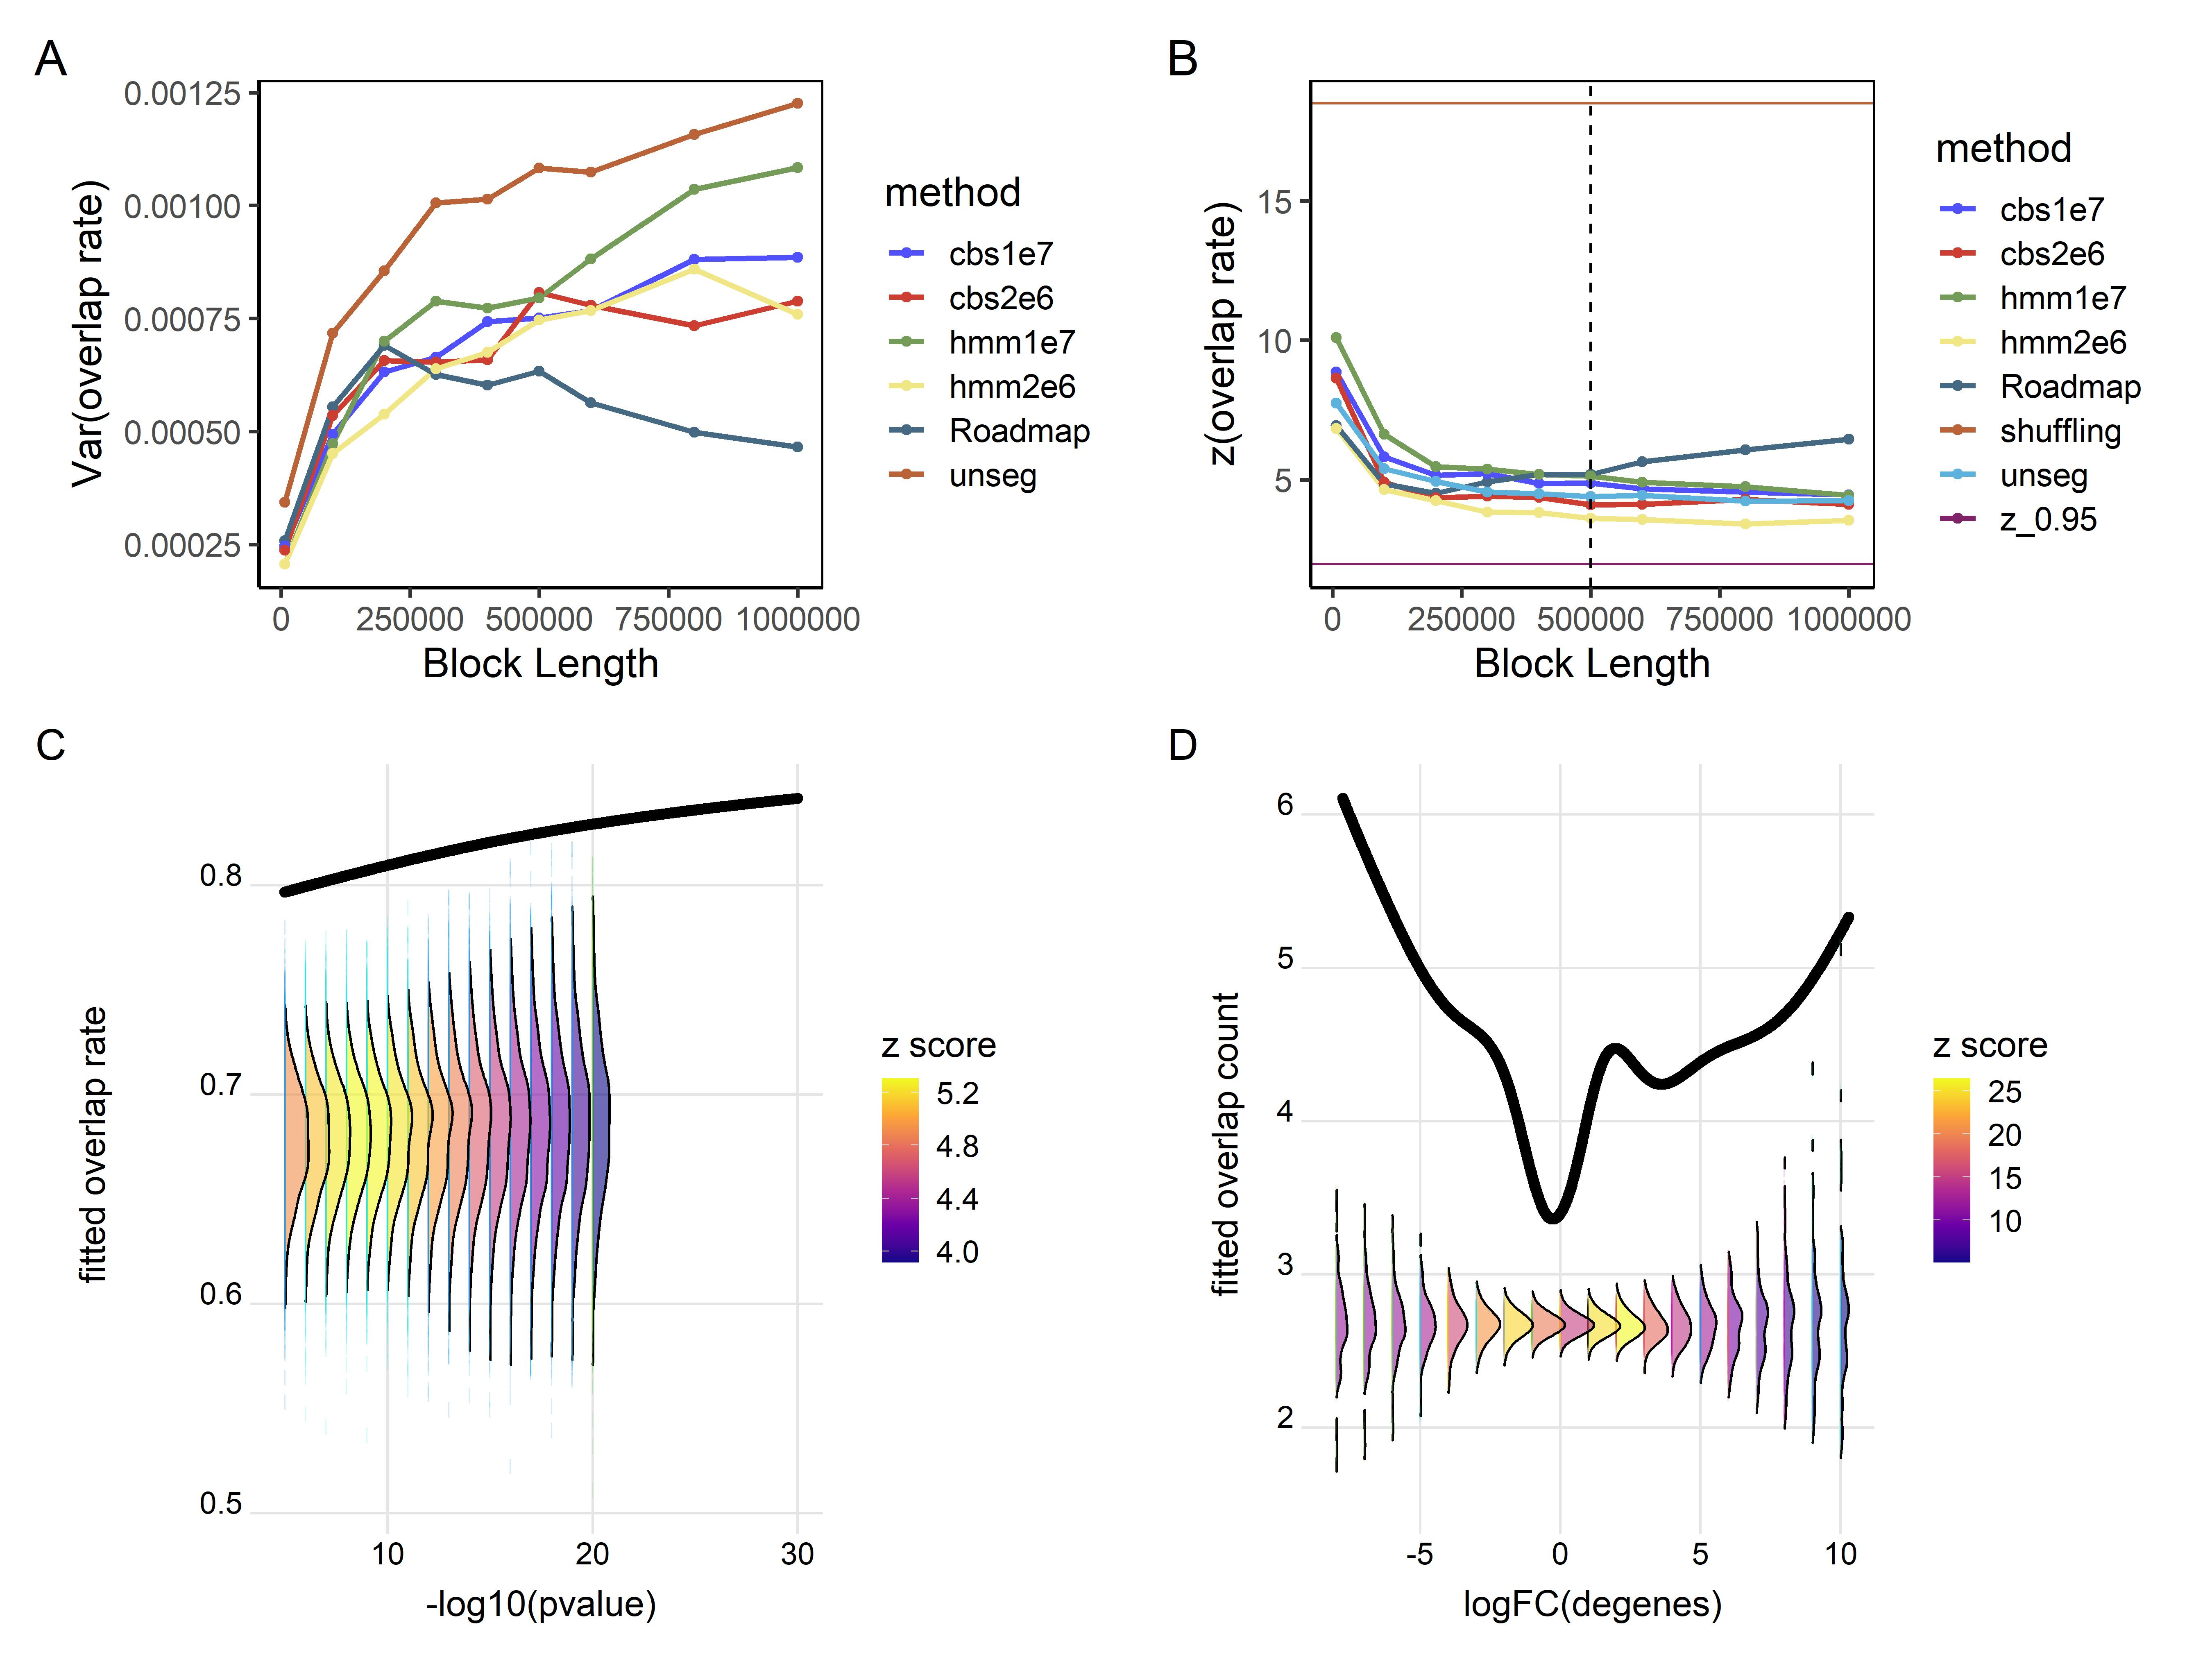
\includegraphics[scale=0.25]{Figures/fig2.jpeg}
\caption{Results of liver caQTL-GWAS(A-C) and macrophage enrichment analysis(D). A) Variance of overlap rate over various segmentation and $L_b$ choice. B) {\it z} score over block length assuming block bootstrap's overlap rate follow Gaussian distribution. Upper and lower horizontal line represents shuffle and upper tailed $z_{0.95}$, separately. C-D) Splines was observsed data's fitted overlap rate over -log10(pvalue) from 5 to 20 or overlap count over log(FC) from -8 to 10. Null sets' fitted value distribution on every integer was plotted by conditional density plot. Color represents the amount of standard deviation(SD) that observed fitted statistics away from null sets' statistics distribution. }
\label{fig:result}
\vspace{-1.2cm}
\end{figure}

The scientific conclusion of this example was there exists a strong association between liver caQTLs and total cholesterol SNPs because of the empirical p value = 0. z score, independent of number of bootstraps, was used to measure the distance between the expected value and the observed one according to the standard deviations.
since the the $z = 4.10$ if look at circular binary search(CBS) \citep{cbs} segmentation method with $L_s = 2e6$ and $L_b=5e5$(\cref{fig:result}B). 
As seen in applications of \citet{bickel2010subsampling}, the effect of segmentation did not greatly alter conclusions, e.g. rejection of the null hypothesis, in this case, although the z score varies greatly among the different segmentations and block lengths.
Genome shuffling (Supplementary \cref{sec:shuffle}) that people usually used when performing such analysis had much higher $z = 18.5$. We believe it may result low specificity in some cases and block bootstrap was, as much as possible, close to actual distribution of genomics elements. 

% As we all known, $5\times 10^{-8}$ was always used as gold standard for GWAS study and stringent logFC threshold are needed sometimes after p value roughly filtration for DEG analysis, but there are no recognized thresholds for those indicators. 
In this study, we showed optimized selection of data driven p-value and logFC through applying \bootranges on pairs of features: 
% caQTL-GWAS for the liver dataset, 
aforementioned example, and chromatin accessibility and gene expression in a macrophage immune response datasets data \citep{alasoo2018shared}. A generalized linear model (GLM) with penalized regression splines from \textit{gam} function in the \emph{mgcv} R package were fitted and \textit{predict\_gam} function in the \emph{tidymv} R package were predicted on observed and each null feature sets. 
$$
\setlength{\abovedisplayskip}{3pt}
\setlength{\belowdisplayskip}{3pt}
log \left( \frac{\pi}{1-\pi} \right) = \beta_0  + f (-log_{10}p), log(\mu) = \beta_0 + f (log_{FC})
$$ 
for rate and count-based statistic, separately. 
%X is all the regulation covariates that want to be accounted for. For simply guidance, we ignored the X in our example.
All generated 95\% percentile intervals at the same time across a range of effect sizes were displayed by conditional density plot (\cref{fig:result} C,D). We found z score was highest when -log10(pvalue)=8 (\cref{fig:suppfig}D) which is quite close to Bonferroni correction and DEG logFC at -2 or 2(\cref{fig:suppfig}E). 
%These numbers gives insight into future study cut-offs. 

%Since genes' expression is most \textit{cis}-regulated by transcription factors which influenced by the chromatin accessibility, there is a belief that two modalities would have significant high correlation across cell types.
We additionally applied
\bootranges to Chromium Single Cell Multiome ATAC + Gene Expression, to assess the correlation of the two modalities for all pairs of genes and promoter peaks, across the 14 cell types (pseudo-bulk).
For the whole gene set, the mean correlation of RNA-seq and ATAC log read counts was 0.33 that was significantly far from the subsampling correlation distribution (\cref{fig:suppfig}F) with expectation 0.007 and empirical value indicated there was significant high correlation between genes expression and open chromatin. Additionally, average gene-promoter correlation per gene can be derived. XXX of genes have a significant higher correlation. 
% Additionally, 5644 significant candidate gene-promoter pairs were identified, among which 5591 genes had only one pair, 25 genes had 2 pairs. By viewing in the UCSC, we found out 
% The most negative correlation gene TET3 had $\rho = -0.963$(\cref{fig:suppfig}G) outside the subsampling 95\% CI [-0.85,0.78]. 


According to the time efficiency, we compared with GSC using the ENCODE kidney and bladder H3K27ac ChIP-seq peaks. The average time to block bootstrap the whole genome using \bootranges is around 0.3s and 0.37s if adding the \plyranges pipeline. While GSC approximate cost 7.56s. Therefore, \bootranges is 20 times faster.
All of the R code and data used in this paper are available at the following repository:
\url{https://github.com/Wancen/bootRangespaper}. 
%So those significant pairs could provide important insights into perturb their corresponding promoter regions for future tumor treatment.
% chr2:74000098-74003475 and chr6:14116971-14139988 for future tumor treatment. 

% Various tidy code pipelines for working with \bootranges can be found in Supplementary \cref{sec:results}. One example for generating bootstrapped correlation is as simple as:

% \begin{lstlisting}[language=R]
% `y'` <- bootRanges(y,blockLength = 5e5, R=100)
% boot_stats<-x %>% join_overlap_inner(`y'`,maxgap=1000) %>%
%   mutate(rho = correlation(counts_x, counts_y)) %>%
%   group_by(iter) %>%
%   summarise(meanRho = mean(rho))
  
% \end{lstlisting} 

\vspace*{-25pt}

\section*{Funding}
This work was funded by a CZI EOSS award to  M.I.L., and a grant to M.I.L. from NIH [NHGRI R01 HG009937].
